%%%%%%%%%%%%%%%%%%%%%%%%%%%%%%%%%%%%%%%%%
% Contract
% LaTeX Template
% Version 1.0 (December 8 2014)
%
% This template has been downloaded from:
% http://www.LaTeXTemplates.com
%
% Original author:
% Brandon Fryslie
% With extensive modifications by:
% Vel (vel@latextemplates.com)
%
% License:
% CC BY-NC-SA 3.0 (http://creativecommons.org/licenses/by-nc-sa/3.0/)
%
% Note:
% If you are using Apple OS X, go into structure.tex and uncomment the font
% specifications for OS X and comment out the default specifications - this will
% drastically increase how good the document looks. You will now need to
% compile with XeLaTeX.
%
%%%%%%%%%%%%%%%%%%%%%%%%%%%%%%%%%%%%%%%%%

\documentclass[usletter, 12pt]{article}
%%%%%%%%%%%%%%%%%%%%%%%%%%%%%%%%%%%%%%%%%
% Contract Structural Definitions File Version 1.0 (December 8 2014)
%
% Created by: Vel (vel@latextemplates.com)
% 
% This file has been downloaded from: http://www.LaTeXTemplates.com
%
% License: CC BY-NC-SA 3.0 (http://creativecommons.org/licenses/by-nc-sa/3.0/)
%
%%%%%%%%%%%%%%%%%%%%%%%%%%%%%%%%%%%%%%%%%

\usepackage{geometry} % Required to modify the page layout
\usepackage{multicol}
\usepackage{amsmath}
\usepackage{amssymb}

\usepackage[pdftex]{graphicx}
\usepackage{wrapfig}
\usepackage[font=scriptsize, labelfont=bf]{caption}
\usepackage[utf8]{inputenc} % Required for including letters with accents
\usepackage[T1]{fontenc} % Use 8-bit encoding that has 256 glyphs

\usepackage{avant} % Use the Avantgarde font for headings
\usepackage{courier}
\usepackage{xparse}
\usepackage{xcolor}
\usepackage{listings}  % for code verbatim and console outputs

\setlength{\textwidth}{16cm} % Width of the text on the page
\setlength{\textheight}{23cm} % Height of the text on the page
\setlength{\oddsidemargin}{0cm} % Width of the margin - negative to move text left, positive to move it right
\setlength{\topmargin}{-1.25cm} % Reduce the top margin

\setlength{\parindent}{0mm} % Don't indent paragraphs
\setlength{\parskip}{2.5mm} % Whitespace between paragraphs
\renewcommand{\baselinestretch}{1.5}

\definecolor{green}{rgb}{0.18, 0.55, 0.34}

\graphicspath{ {figures/} }
\captionsetup[table]{skip=10pt}

\lstset{language=C, keywordstyle={\bfseries \color{black}}}

% defines algorithm counter for chapter-level
\newcounter{nalg}[section]

%defines appearance of the algorithm counter
\renewcommand{\thenalg}{\thesection .\arabic{nalg}}

% defines a new caption label as Algorithm x.y
\DeclareCaptionLabelFormat{algocaption}{Algorithm \thenalg}

% defines the algorithm listing environment
\lstnewenvironment{pseudocode}[1][] {
    \refstepcounter{nalg}  % increments algorithm number
    \captionsetup{font=normalsize, labelformat=algocaption, labelsep=colon}
    \lstset{
        breaklines=true,
        mathescape=true,
        numbers=left,
        numberstyle=\scriptsize,
        basicstyle=\footnotesize\ttfamily,
        keywordstyle=\color{black}\bfseries,
        keywords={input, output, return, parallel, function, for, to, in, if,
        else, foreach, while, and, or, new, print},
        xleftmargin=.04\textwidth,
        #1
    }
}{}

\renewcommand{\familydefault}{\sfdefault}  % default font for entire document
 % Input the structure.tex file which specifies the document layout and style

%----------------------------------------------------------------------------------------
%   DYNAMIC CONTRACT INFORMATION
%----------------------------------------------------------------------------------------

% Member's information
\newcommand{\project}{Homework - Mastermind}
\newcommand{\Sabbir}{Sabbir Ahmed}

%----------------------------------------------------------------------------------------

\begin{document}

    %----------------------------------------------------------------------------------------
    %   TITLE PAGE
    %----------------------------------------------------------------------------------------

    \begin{titlepage}

        \vspace*{\fill} % Add whitespace above to center the title page content
        \begin{center}

            {\LARGE \project~Report Draft}\\ [1.5cm]

            Submitted: \today
            
            \vspace*{\fill}

            \Sabbir

        \end{center}
        \vspace*{\fill} % Add whitespace below to center the title page content

    \end{titlepage}

    \section{Description}

        This project emulates a variant of the game "mastermind" on the AVR Dragon. The user will take guesses at the code using the joystick with combinations of up-down-left-right. A wrong input will sound a buzzer (piezoelectric element) and reset the user’s game. Completing the code will light an LED. At this point the game can be reset by pressing the push-button. All inputs will be logged over a serial interface (UART) to a computer reporting the state of the game.

    \section{State Machine Implementation}

        The game is implemented as a state machine, where each successful inputs progresses through the states.

        \begin{figure}[ht]
            \begin{center}
                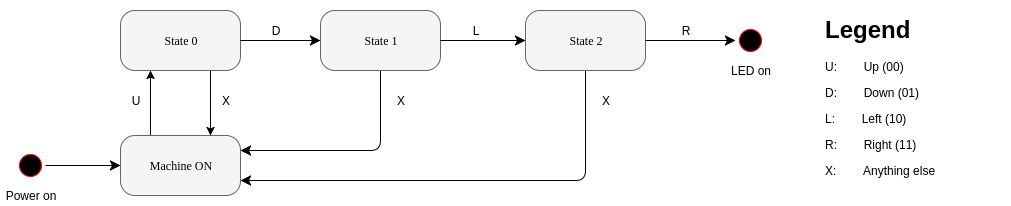
\includegraphics[width=1\textwidth]{state_diagram.png}
                \caption{State Diagram Implementation of the Game} \label{fig:state_diagram}
            \end{center}
        \end{figure}

    \section{Code}

        The assembly code used for the implementation has been attached and provided at the end of the report.

        \subsection{mastermind.asm}
        Contains the state machine implementation of the game.

        \subsection{uart.asm}
        Contains the specifications for the UART interface.

    \newpage
    \VerbatimInput{mastermind.asm}

    \newpage
    \VerbatimInput{uart.asm}


\end{document}
